\section{Evaluation}
\newcommand{\EvaluationTitle}{Evaluation}
\begin{frame}[fragile]
    \frametitle{\EvaluationTitle}
    \subsection{Setup}
    \framesubtitle{Setup}
    Graph file simulation\\
    \begin{itemize}%[<+->]
        \item Full input - output
        \item Does not take latency between packets into account
        \item Simplifies test cases
    \end{itemize}
\end{frame}
\note{Definer send og receive bedre}


\begin{frame}[fragile]
    \frametitle{\EvaluationTitle}
    \framesubtitle{Setup}
    \begin{columns}
        \begin{column}{0.45\textwidth}
            \centering
            Graph simulation node types\\
            \begin{figure}
                \centering
                \begin{minipage}{0.33\textwidth}
                    \centering
                    \includegraphics[scale=0.45]{evaluation/dot_files/datain.eps}
                    Data In
                    \label{fig:packet_graph_datain}
                \end{minipage}%
                \begin{minipage}{0.33\textwidth}
                    \centering
                    
\includegraphics[scale=0.45]{evaluation/dot_files/send.eps}
                    Send
                    \label{fig:packet_graph_send}
                \end{minipage}%
                \begin{minipage}{0.33\textwidth}
                    \centering
                    \includegraphics[scale=0.45]{evaluation/dot_files/command.eps}
                    Command
                    \label{fig:packet_graph_command}
                \end{minipage}%
                \\
                \begin{minipage}{0.33\textwidth}
                    \centering
                    \includegraphics[scale=0.45]{evaluation/dot_files/dataout.eps}
                    Data Out
                    \label{fig:packet_graph_dataout}
                \end{minipage}%
                \begin{minipage}{0.33\textwidth}
                    \centering
                    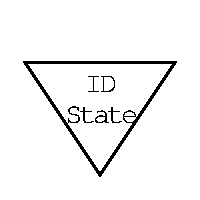
\includegraphics[scale=0.45]{evaluation/dot_files/receive.eps}
                    Receive
                    \label{fig:packet_graph_receive}
                \end{minipage}%
                \begin{minipage}{0.33\textwidth}
                    \centering
                    \includegraphics[scale=0.45]{evaluation/dot_files/wait.eps}
                    Wait
                    \label{fig:packet_graph_wait}
                \end{minipage}%
            \end{figure}%
        \end{column}
        \begin{column}{0.55\textwidth}
            {\renewcommand{\arraystretch}{1.5}
            \begin{table}
                \begin{center}
                    \begin{tabular}{lc}
                        State and Color &Description\\ \hline \hline
                        \statecolorboxtext{graph_waiting}{Waiting} &
                        \makecell{Vertex is not in use.}\\ \hline

                        \statecolorboxtext{graph_isready}{Ready} &
                        \makecell{Vertex Is ready\\ for activation.}\\ \hline

                        \statecolorboxtext{graph_active}{Active} &
                        \makecell{Vertex is active.\\ Simulator is\\ gathering data.}\\ \hline

                        \statecolorboxtext{graph_inactive}{Inactive} &
                        \makecell{Vertex is inactive.\\Simulator is not\\ gathering data.}\\ \hline

                        \statecolorboxtext{graph_done}{Done} &
                        \makecell{Vertex is done\\ and validated.}
                    \end{tabular}
                \end{center}
            \end{table}
            }
        \end{column}
    \end{columns}
\end{frame}

\begin{frame}[fragile]%
    \frametitle{\EvaluationTitle}
    \framesubtitle{Setup}
    \begin{columns}%
        \begin{column}{0.50\textwidth}
            \begin{figure}
            \centering
                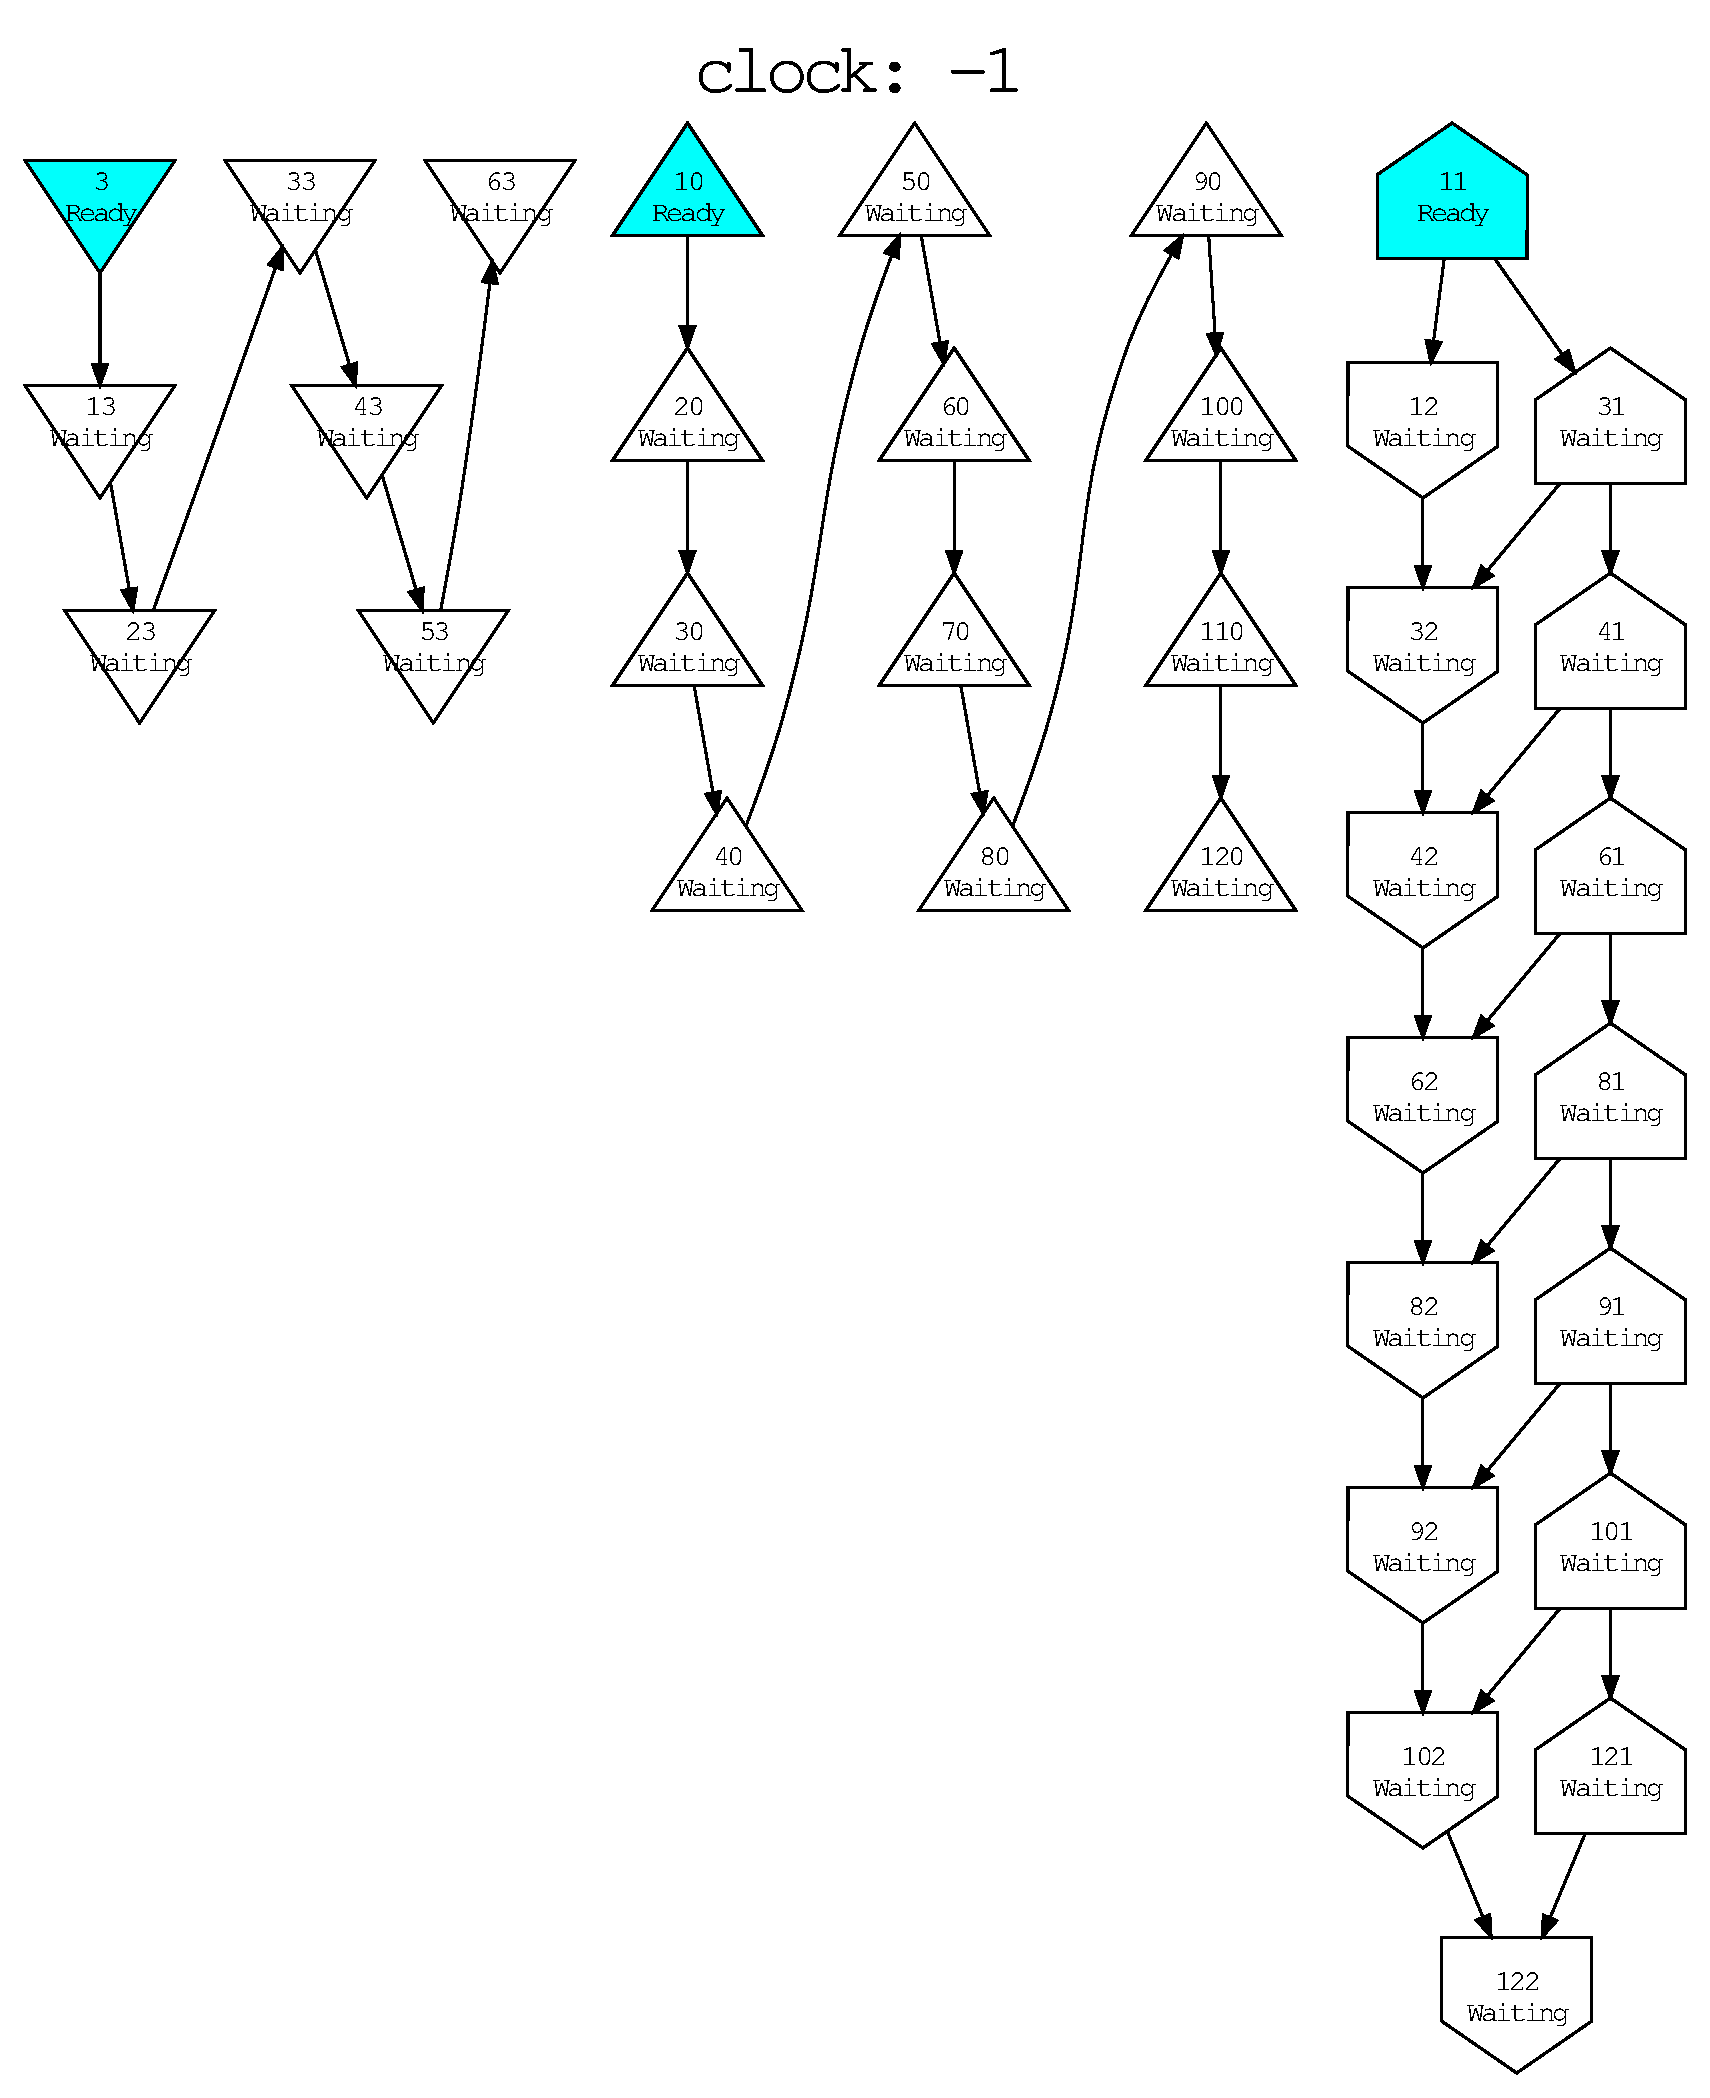
\includegraphics[scale=0.21]{evaluation/dot_files/example_graph_initial_compact.eps}
                \caption{The initial state of a simulation}
            \end{figure}
        \end{column}%
        \begin{column}{0.50\textwidth}
            \begin{figure}
                \centering
                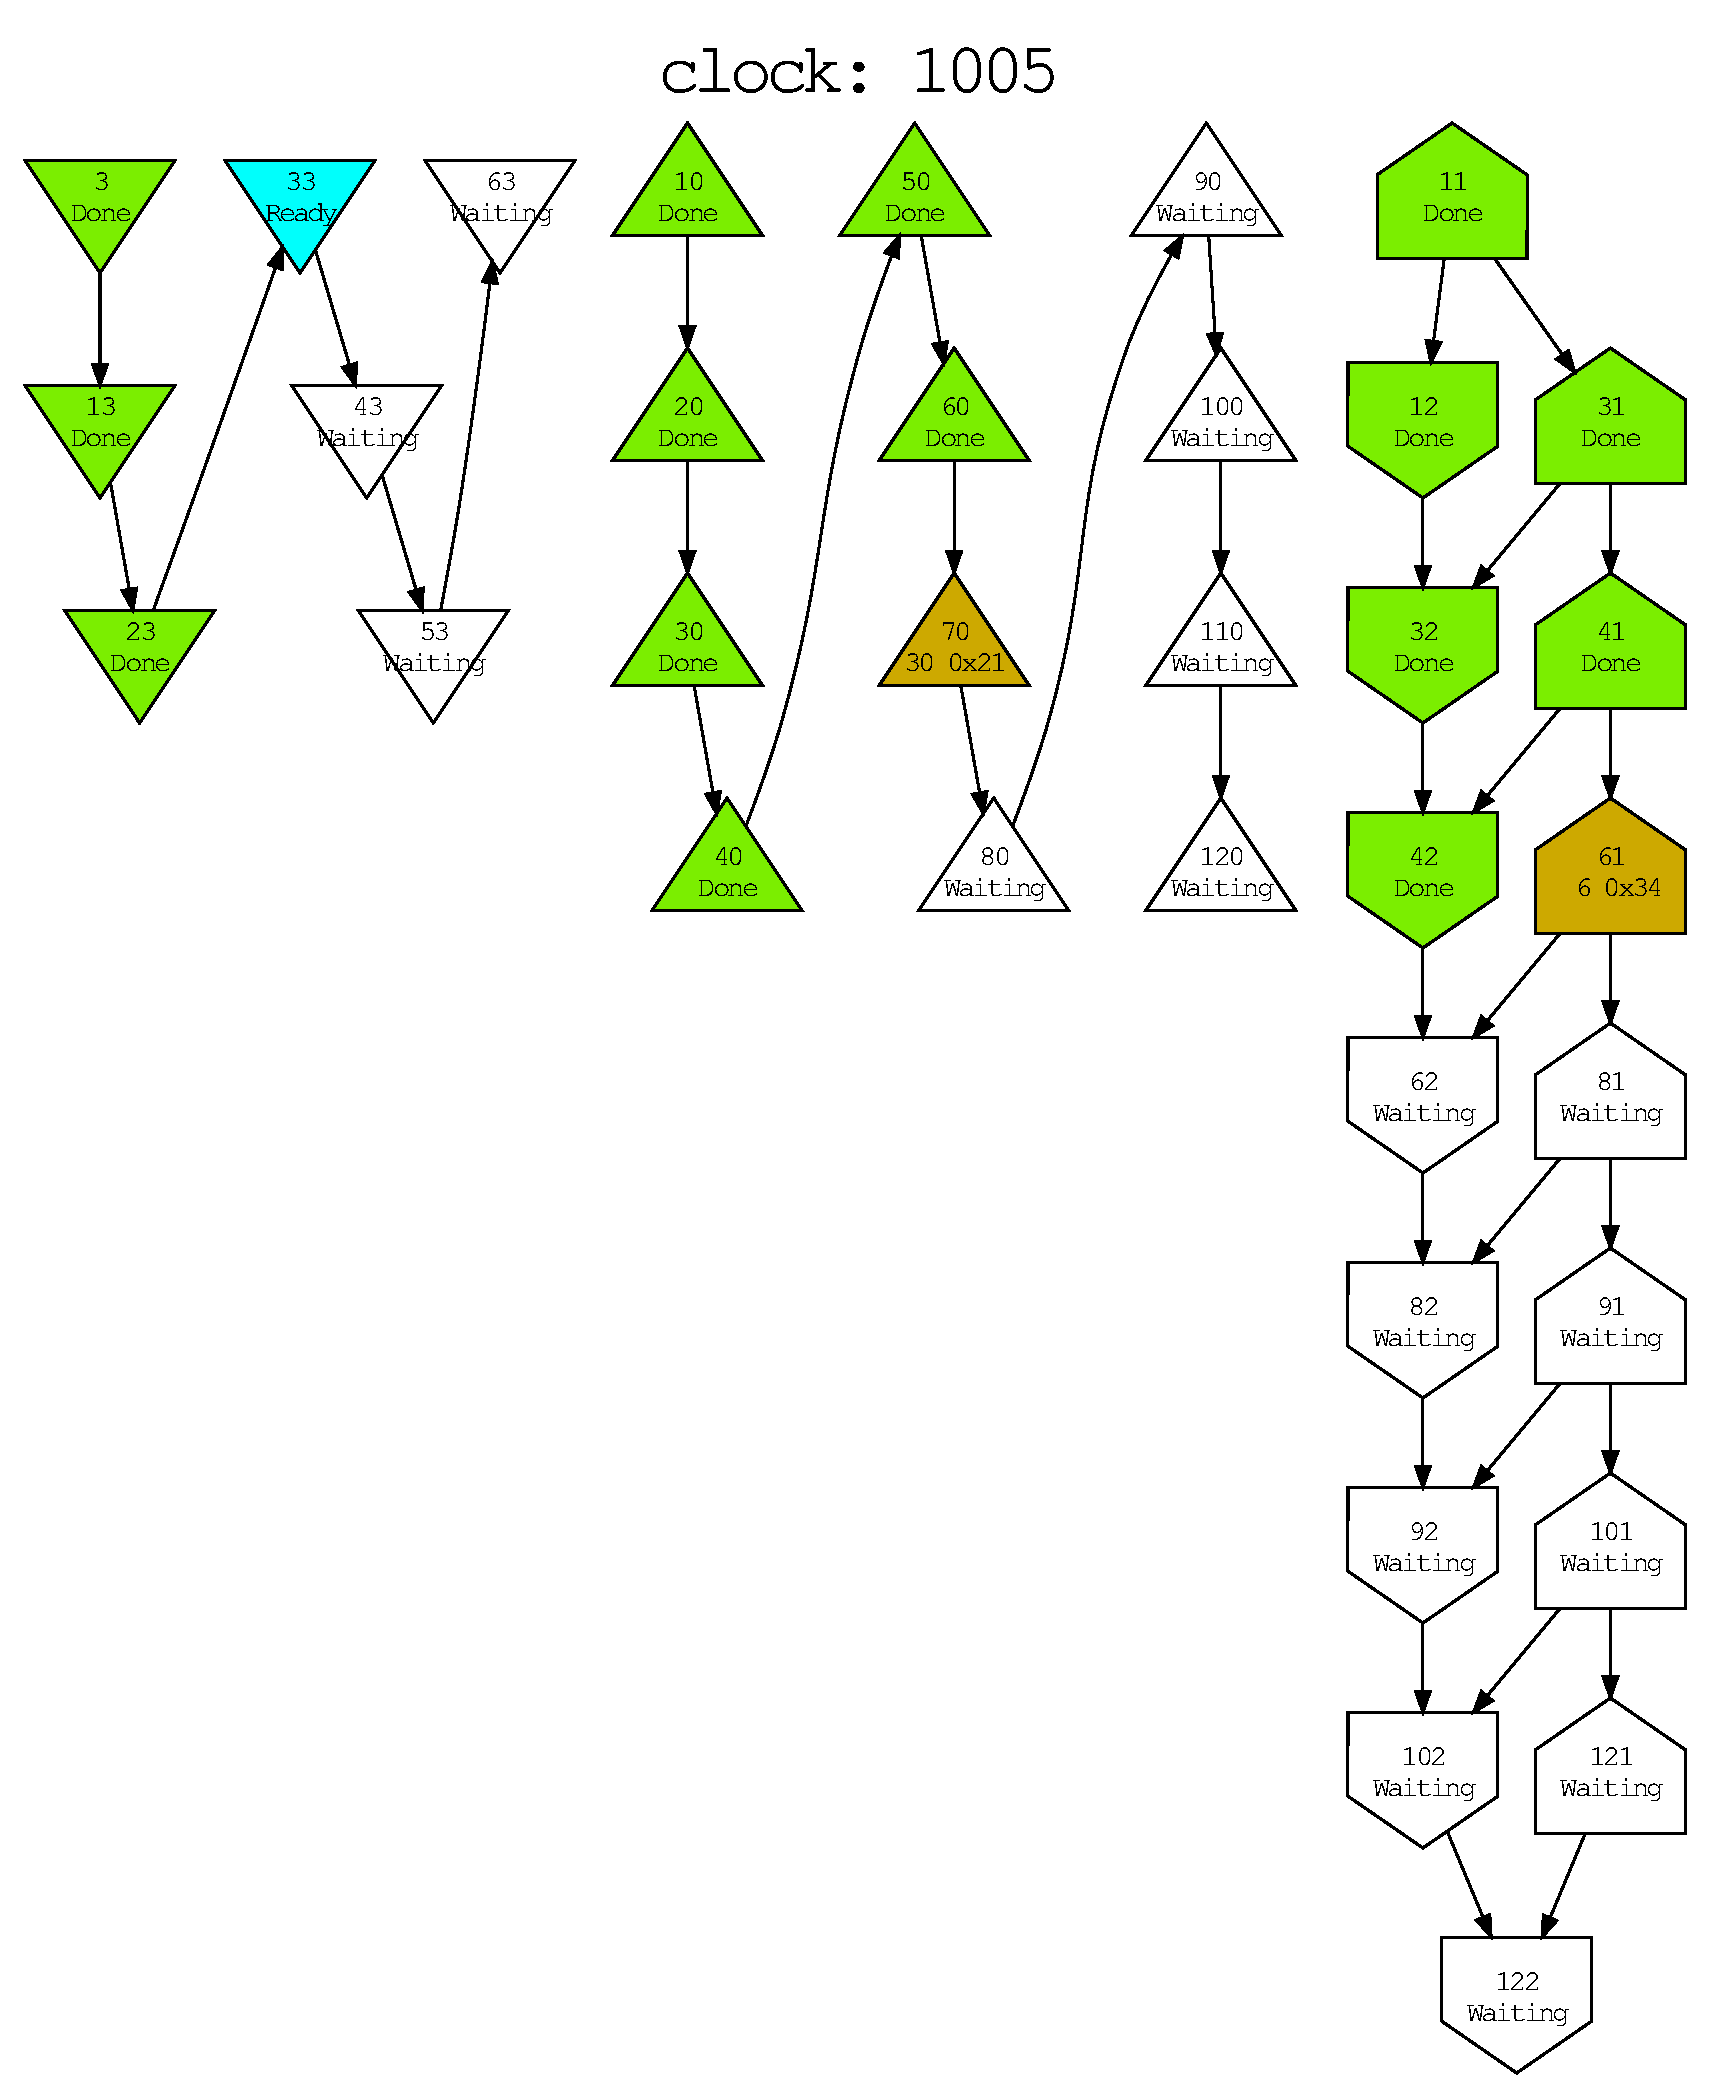
\includegraphics[scale=0.21]{evaluation/dot_files/example_graph_running_compact.eps}
                \caption{The state after 1005 clocks}
            \end{figure}
        \end{column}
    \end{columns}
\end{frame}

\begin{frame}%
    \frametitle{\EvaluationTitle}
    \subsection{Test}
    \framesubtitle{Test}
    Senario
    \begin{itemize}%[<+->]
        \item Real life scenario
        \item Test at high workloads
        \item Remove garbage
        \item Respond to packet
        \item Differ between concurrent connections
    \end{itemize}
\end{frame}

\begin{frame}%
    \frametitle{\EvaluationTitle}
    \framesubtitle{Test}
    The test
    \begin{itemize}%[<+->]
        \item 17283 packets in total
        \item Two "sessions"
        \item 640*2 UDP packets that needs a response
        \item 640 well formed UDP packets with no session (discard)
        \item Rest of data is "background noise" (TCP packets with state, data, etc)
        \item Total data sent through: 1832958 bytes
        \item ~1.83 Million clocks used
    \end{itemize}
\end{frame}

\begin{frame}%
    \frametitle{\EvaluationTitle}
    \subsection{Validation}
    \framesubtitle{Validation}
    Latency calculations:
    \begin{columns}
        \begin{column}{0.60\textwidth}
            \begin{description}[$n_{\mathtt{T}}$]
                \item[$n_{\mathtt{D}}$]:
                The number of bytes in the data part of the protocol. This excludes both
                headers from transport and internet.
                \item[$n_{\mathtt{I}}$]:
                The internet header size.
                \item[$n_{\mathtt{T}}$]:
                The transport header size.
                \item[$n$]:\quad
                The total packet size.
            \end{description}
        \end{column}
        \begin{column}{0.40\textwidth}
            From packet to user
            \begin{equation*}
                6 + n_{\mathtt{I}} + 2n_{\mathtt{T}} + 3n_{\mathtt{D}}
           \end{equation*}\\
           \noindent\rule{8cm}{0.4pt}
           From user to packet
           \begin{equation*}
            8 + 2n_{\mathtt{I}} + 3n_{\mathtt{T}} + 4n_{\mathtt{D}}
            \end{equation*}
        \end{column}
    \end{columns}
\end{frame}
\note{Hav billede af sytem ved siden af\\
system graf med selve latency\\ bufferen kan ikke videresende data dirrekte, da den skal
gemme segmentet først}

\begin{frame}%
    \frametitle{\EvaluationTitle}
    \framesubtitle{Validation}
    Outgoing packet validation:
    \begin{figure}
        \centering
        \includegraphics[scale=0.33]{evaluation/hexdump.pdf}
    \end{figure}
\end{frame}
\note{Protocol ikke sat korrekt, destination ip ikke sat korrekt}


\begin{frame}%
    \frametitle{\EvaluationTitle}
    \framesubtitle{Validation}
    Internet Protocol Suite compliancy as per RFC 1122
\end{frame}
\note{Ikke testet helt igennem, mem felterne er generelt sat}
